% Copyright (c) 2015 Daniele Masini - d.masini.it@gmail.com
% Copyright (c) 2016 Daniele Zambelli - daniele.zambelli@gmail.com

\chapter{Rette parallele}
\label{chap:rette_parallele}

% \includegraphics[width=0.95\textwidth]
% {\folder img/intersection_de_deux_paralleles.jpg}
% \begin{center}
%   {\large ``Intersection de deux parallèles''}\par
%   Foto di OliBac\par
%   \url{http://www.flickr.com/photos/olibac/3244014009/}\par
%   Licenza: Creative Commons Attribution\par
% \end{center}
% \newpage

\section{Rette parallele}\label{sect:rette_parallele}

Secondo la definizione di Euclide, due rette nel piano sono parallele 
se non hanno punti in comune.
In maniera più moderna il concetto di parallelismo è interpretato 
come l'avere la stessa direzione.
Si può anche dare una formulazione che unifichi le due definizioni 
precedenti; si deve però ricorrere al concetto di distanza: due rette 
nel piano sono parallele se mantengono sempre la stessa distanza. Se 
la distanza è nulla, le due rette sono coincidenti.
Noi utilizzeremo la seguente:
\begin{definizione}
  Due rette giacenti nello stesso piano si dicono \emph{parallele} se 
  sono coincidenti oppure non si incontrano mai.
\end{definizione}

Assumendo dunque questa come definizione di parallelismo, abbiamo 
bisogno di precisare il concetto di distanza.
Dati due punti $P$ e $Q$, la \emph{distanza} tra $P$ e $Q$ è la 
lunghezza del \emph{percorso più breve} che unisce i due punti. 
Questo concetto è valido anche se si riferisce alle distanze tra due 
città che si trovano negli stradari: sono riportate le lunghezze dei 
percorsi minimi tra tutte le strade alternative che collegano due 
città. Naturalmente, nel piano, ove si ``dispone'' di tutti i punti 
da poter ``attraversare'', il percorso più breve che collega due 
punti $P$ e $Q$ è il segmento $PQ$; quindi nella geometria euclidea 
assumiamo come distanza tra due punti la lunghezza del segmento 
avente per estremi i due punti.

Se vogliamo parlare di distanza tra due insiemi di punti, allora va 
considerato il percorso più breve tra tutti i percorsi che collegano 
un qualsiasi punto del primo insieme con un qualsiasi punto del 
secondo: in pratica la distanza è la lunghezza del più piccolo 
segmento tra tutti quelli che collegano i due insiemi di punti. 

Nel caso particolare di un punto $A$ ed una retta $BC$, se il punto 
appartiene alla retta allora la distanza di $A$ da $BC$ è uguale a 
zero, altrimenti si considera come distanza la lunghezza del segmento 
$AH$, dove $H$ è il punto in cui la perpendicolare a $BC$ passante 
per $A$ interseca la stessa retta $BC$: il motivo si intuisce in base 
a quanto detto, ma risulterà chiaro più avanti, quando affronteremo 
lo studio delle disuguaglianze tra gli elementi di un triangolo. 

Analogamente, come distanza tra due rette parallele si assume la 
lunghezza di un qualunque segmento che unisce il punto di una delle 
due rette con il piede della perpendicolare mandata da esso 
sull'altra retta. Affermare che tali segmenti sono tutti congruenti è 
un modo più preciso per dire che le due rette mantengono sempre la 
stessa distanza.

Ricordiamo la versione ``moderna'' del V Postulato di Euclide: 
\emph{dati una retta $r$ ed un punto $P$, allora esiste una ed una 
  sola retta parallela ad $r$ e passante per $P$.}

Si è scelto di considerare 
parallele sia rette nel piano che non hanno punti in comune sia rette 
coincidenti proprio per fare in modo che la relazione di parallelismo 
sia una relazione di equivalenza: riflessiva, simmetrica, transitiva. 
Con la definizione di parallelismo data da Euclide, al contrario, 
sarebbe stata solo simmetrica, ma non riflessiva né transitiva. Per 
convincersi della non transitività, basta considerare tre rette $a$, 
$b$, $c$ con $a$ e $c$ coincidenti e $b$ parallela ad entrambe e 
distinta da esse: allora $a\parallel b$ e $b \parallel c$, ma $a$ e 
$c$ non sono parallele secondo la definizione di Euclide.

\begin{procedura}
  Costruzione della parallela a una retta, passante per un punto C esterno ad 
essa:
  \begin{enumerate} [nosep]
    \item 
    Traccia la retta r  passante per due punti qualsiasi A e B.
    \item 
    Traccia un punto C non appartenente alla retta.
    \item 
    Traccia la retta passante per C ed A. 
    \item 
    Traccia la circonferenza C\_0 di centro C e raggio CA  
    \item       
    Traccia la circonferenza C\_1 di centro A e raggio CA
    \item   
    Denomina D ed E (E è più vicino a C) i punti di intersezione della retta r 
con la circonferenza C\_1.  
    \item 
    Traccia la circonferenza C\_2 di centro A e raggio EC, che 
interseca la circonferenza C\_1 nei punti G ed F (G appartiene allo stesso 
semipiano individuato da r, contenente C).
    \item
    Traccia la retta CG, che è la parallela alla retta AB, passante per C.
  \end{enumerate}
\end{procedura}

\subsection{Rette parallele tagliate da una trasversale}

Due rette parallele $a$ e $b$ vengono intersecate da una retta $c$ 
(detta \emph{trasversale}) che non è parallela ad esse,
\begin{itemize*}
  \item se la retta $c$ è perpendicolare (ad entrambe), si vengono a 
  formare otto angoli retti; 
  \item se la retta $c$ non è perpendicolare ad esse, si vengono a 
  formare otto angoli, di cui quattro acuti e quattro ottusi, rispetto 
  alla posizione che occupano alle coppie vengono attribuiti i seguenti 
  nomi (figura~\ref{fig:rette_parall_2}):
  \begin{itemize*}
    \item le coppie di angoli 1 e 5, 2 e 6, 3 e 7, 4 e 8 si dicono 
    \emph{corrispondenti} (perché occupano posizioni analoghe da una 
    parallela all'altra);
    \item le coppie di angoli 3 e 5, 4 e 6 si dicono \emph{alterni 
      interni} (alterni perché occupano posizioni opposte rispetto alla 
    trasversale, interni perché si trovano all'interno delle due 
    parallele);
    \item le coppie di angoli 1 e 7, 2 e 8 si dicono \emph{alterni 
      esterni} (alterni perché sono opposti rispetto alla trasversale; 
    esterni perché si trovano all'esterno della zona tra le due 
    parallele);
    \item le coppie di angoli 3 e 6, 4 e 5 si dicono \emph{coniugati 
      interni} (si dicono coniugati perché stanno dalla stessa parte 
    rispetto alla trasversale);
    \item le coppie di angoli 1 e 8, 2 e 7 si dicono \emph{coniugati 
      esterni}.
  \end{itemize*}
\end{itemize*}
Inoltre le coppie 1 e 3, 2 e 4, 5 e 7, 6 e 8 sono angoli opposti al 
vertice.


\begin{inaccessibleblock}[Figura: TODO]
  \begin{figure}[htb]
    \centering% Copyright (c) 2015 Daniele Masini - d.masini.it@gmail.com

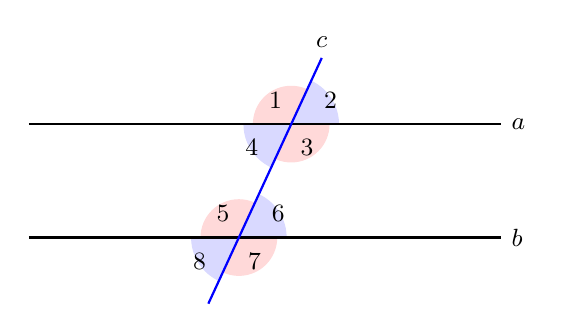
\begin{tikzpicture}[scale=1.2,font=\small, dot/.style={circle,inner sep=1pt, fill, label={#1}, name=#1}, extended line/.style={shorten >=-#1,shorten <=-#1}, extended line/.default=1cm]
\usetikzlibrary{calc, intersections}

\begin{scope}

\coordinate (a1) at (-2.5,0);
\coordinate (a2) at (2.5,0);
\coordinate (b1) at (-2.5,-1.2);
\coordinate (b2) at (2.5,-1.2);

\coordinate (c1) at (0.6,0.7);
\coordinate (c2) at (-0.6,-1.9);

\coordinate (p1) at (intersection of c1--c2 and a1--a2);
\coordinate (p2) at (intersection of c1--c2 and b1--b2);

\begin{scope}
\clip (a1) -- (p1) -- (c1) -- cycle;
\draw[fill, red!15] (p1) circle (0.4) node[shift={(-0.2,0.3)}, black] {1};
\end{scope}

\begin{scope}
\clip (a2) -- (p1) -- (c1) -- cycle;
\draw[fill, blue!15] (p1) circle (0.5) node[shift={(0.5,0.3)}, black] {2};
\end{scope}

\begin{scope}
\clip (a2) -- (p1) -- (c2) -- cycle;
\draw[fill, red!15] (p1) circle (0.4) node[shift={(0.2,-0.3)}, black] {3};
\end{scope}

\begin{scope}
\clip (a1) -- (p1) -- (c2) -- cycle;
\draw[fill, blue!15] (p1) circle (0.5) node[shift={(-0.5,-0.3)}, black] {4};
\end{scope}

\begin{scope}
\clip (b1) -- (p2) -- (c1) -- cycle;
\draw[fill, red!15] (p2) circle (0.4) node[shift={(-0.2,0.3)}, black] {5};
\end{scope}

\begin{scope}
\clip (b2) -- (p2) -- (c1) -- cycle;
\draw[fill, blue!15] (p2) circle (0.5) node[shift={(0.5,0.3)}, black] {6};
\end{scope}

\begin{scope}
\clip (b2) -- (p2) -- (c2) -- cycle;
\draw[fill, red!15] (p2) circle (0.4) node[shift={(0.2,-0.3)}, black] {7};
\end{scope}

\begin{scope}
\clip (b1) -- (p2) -- (c2) -- cycle;
\draw[fill, blue!15] (p2) circle (0.5) node[shift={(-0.5,-0.3)}, black] {8};
\end{scope}

\draw[thick] (a1)--(a2) node[right] {$a$};
\draw[thick] (b1)--(b2) node[right] {$b$};
\draw[thick, blue] (c1) node[above, black] {$c$} --(c2);

\end{scope}


\end{tikzpicture}

    \caption{Le rette parallele $a$ e $b$ sono tagliate dalla trasversale 
      $c$}\label{fig:rette_parall_2}
  \end{figure}
\end{inaccessibleblock}

\begin{teorema}[delle parallele {[}diretto{]}]
  Se due rette tagliate da una trasversale formano una coppia di angoli 
  alterni interni congruenti allora sono parallele.
\end{teorema}


\begin{inaccessibleblock}[Figura: TODO]
  \begin{figure}[htb]
    \centering% Copyright (c) 2015 Daniele Masini - d.masini.it@gmail.com

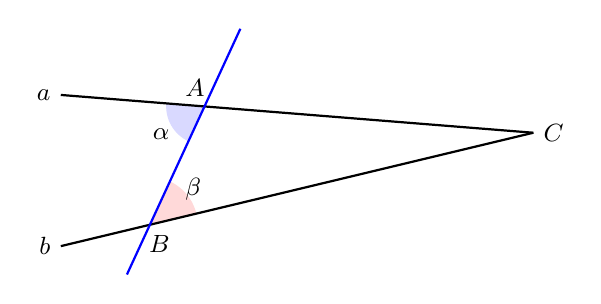
\begin{tikzpicture}[scale=1.2,font=\small, dot/.style={circle,inner sep=1pt, fill, label={#1}, name=#1}, extended line/.style={shorten >=-#1,shorten <=-#1}, extended line/.default=1cm]
\usetikzlibrary{calc, intersections}

\begin{scope}

\coordinate (a1) at (-2.5,0);
\coordinate (a2) at (2.5,-0.4);
\coordinate (b1) at (-2.5,-1.6);
\coordinate (b2) at (2.5,-0.4);

\coordinate (c1) at (-0.6,0.7);
\coordinate (c2) at (-1.8,-1.9);

\coordinate (p1) at (intersection of c1--c2 and a1--a2);
\coordinate (p2) at (intersection of c1--c2 and b1--b2);

\begin{scope}
\clip (a1) -- (p1) -- (c2) -- cycle;
\draw[fill, blue!15] (p1) circle (0.4) node[shift={(-0.55,-0.35)}, black] {$\alpha$};
\end{scope}

\begin{scope}
\clip (b2) -- (p2) -- (c1) -- cycle;
\draw[fill, red!15] (p2) circle (0.5) node[shift={(0.55,0.45)}, black] {$\beta$};
\end{scope}

\draw[thick] (a1) node[left] {$a$} --(a2) node[right] {$C$};
\draw[thick] (b1) node[left] {$b$}--(b2) ;
\draw[thick,blue] (c1) -- (c2);
\node at ([shift={(-0.1,0.2)}]p1) {$A$};
\node at ([shift={(0.1,-0.2)}]p2) {$B$};

\end{scope}


\end{tikzpicture}

  \end{figure}
\end{inaccessibleblock}

\begin{proof}
  Ragioniamo per assurdo. Supponiamo che la tesi sia falsa, cioè che le 
  rette $a$ e $b$ non siano parallele. Se non sono parallele si 
  incontreranno in un punto $C$ e quindi tra esse e la trasversale si 
  viene a formare il triangolo $ABC$. Per il teorema dell'angolo 
  esterno del triangolo, l'angolo (esterno) $\alpha$ è maggiore 
  dell'angolo (interno) $\beta$. Questa conseguenza contraddice 
  l'ipotesi del teorema, secondo la quale gli angoli alterni interni 
  $\alpha$ e $\beta$ sono congruenti. Allora abbiamo sbagliato a negare 
  la tesi, che perciò risulta vera.
\end{proof}

Possiamo generalizzare il teorema precedente ad altri casi.
\begin{teorema}[Criterio di parallelismo]
  Se due rette tagliate da una trasversale danno origine ad una tra le 
  seguenti coppie di angoli
  \begin{itemize*}
    \item angoli alterni interni o alterni esterni congruenti;
    \item angoli corrispondenti congruenti;
    \item angoli coniugati interni o coniugati esterni supplementari
  \end{itemize*}
  allora sono parallele.
\end{teorema}

\noindent \begin{minipage}{0.7\textwidth}
  \begin{proof}
    Tenendo conto che due angoli opposti al vertice sono congruenti e due 
    angoli adiacenti sono supplementari, se risulta che due angoli 
    corrispondenti qualsiasi sono congruenti, allora i quattro angoli 
    acuti sono tutti congruenti ed i quattro angoli ottusi sono 
    congruenti, e quindi anche angoli alterni interni. Pertanto, per il 
    teorema precedente, le rette sono parallele.
    
    \hspace{15pt}Analogamente, se risultano supplementari due qualsiasi 
    angoli coniugati (interni o esterni) risulta sempre che i quattro 
    angoli acuti sono tutti congruenti tra loro come i quattro angoli 
    ottusi, pertanto gli angoli alterni interni sono congruenti e, sempre 
    per il teorema precedente, le due rette sono parallele.
  \end{proof}
\end{minipage}\hfil
\begin{minipage}{0.3\textwidth}
  \centering% Copyright (c) 2015 Daniele Masini - d.masini.it@gmail.com

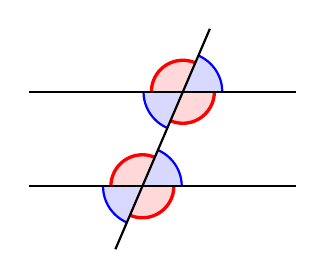
\begin{tikzpicture}[scale=1,font=\small, dot/.style={circle,inner sep=1pt, fill, label={#1}, name=#1}, extended line/.style={shorten >=-#1,shorten <=-#1}, extended line/.default=1cm]
\usetikzlibrary{calc, intersections}

\begin{scope}

\coordinate (a1) at (-1.7,0);
\coordinate (a2) at (1.7,0);
\coordinate (b1) at (-1.7,-1.2);
\coordinate (b2) at (1.7,-1.2);

\coordinate (c1) at (0.6,0.8);
\coordinate (c2) at (-0.6,-2);

\coordinate (p1) at (intersection of c1--c2 and a1--a2);
\coordinate (p2) at (intersection of c1--c2 and b1--b2);

\begin{scope}
\clip (a1) -- (p1) -- (c1) -- cycle;
\draw[very thick, red, fill=red!15] (p1) circle (0.4);
\end{scope}

\begin{scope}
\clip (a2) -- (p1) -- (c1) -- cycle;
\draw[thick, blue, fill=blue!15] (p1) circle (0.5);
\end{scope}

\begin{scope}
\clip (a2) -- (p1) -- (c2) -- cycle;
\draw[very thick, red, fill=red!15] (p1) circle (0.4);
\end{scope}

\begin{scope}
\clip (a1) -- (p1) -- (c2) -- cycle;
\draw[thick, blue, fill=blue!15] (p1) circle (0.5);
\end{scope}

\begin{scope}
\clip (b1) -- (p2) -- (c1) -- cycle;
\draw[very thick, red, fill=red!15] (p2) circle (0.4);
\end{scope}

\begin{scope}
\clip (b2) -- (p2) -- (c1) -- cycle;
\draw[thick, blue, fill=blue!15] (p2) circle (0.5);
\end{scope}

\begin{scope}
\clip (b2) -- (p2) -- (c2) -- cycle;
\draw[very thick, red, fill=red!15] (p2) circle (0.4);
\end{scope}

\begin{scope}
\clip (b1) -- (p2) -- (c2) -- cycle;
\draw[thick, blue, fill=blue!15] (p2) circle (0.5);
\end{scope}

\draw[thick] (a1)--(a2);
\draw[thick] (b1)--(b2);
\draw[thick] (c1) --(c2);

\end{scope}


\end{tikzpicture}

\end{minipage}

\begin{teorema}[delle parallele {[}inverso{]}]
  Se due rette sono parallele allora esse formano con una trasversale 
  qualsiasi due angoli alterni interni congruenti.
\end{teorema}

\noindent \begin{minipage}{0.6\textwidth}
  \begin{proof}
    Ragioniamo per assurdo. Supponiamo che la tesi sia falsa, cioè che 
    esista una coppia di angoli alterni interni $\alpha$ e $\beta$ con 
    $\alpha>\beta$. Per il punto $P$, vertice dell'angolo $\alpha$ si 
    potrà allora tracciare una retta $a'$ in modo che l'angolo da essa 
    formato $\alpha'$ sia congruente a $\beta$. Ne segue che $a'$ e $b$ 
    sono parallele perché formano angoli alterni interni congruenti. 
    Allora esisterebbero due rette distinte, $a$ e $a'$, passanti per lo 
    stesso punto $P$, entrambe parallele alla retta $b$. Questa 
    conclusione contraddice il V postulato di Euclide, secondo il quale 
    per un punto esterno a una retta passa un'unica parallela. In altre 
    parole la tesi è vera.
  \end{proof}
\end{minipage}\hfil
\begin{minipage}{0.4\textwidth}
  \centering% Copyright (c) 2015 Daniele Masini - d.masini.it@gmail.com

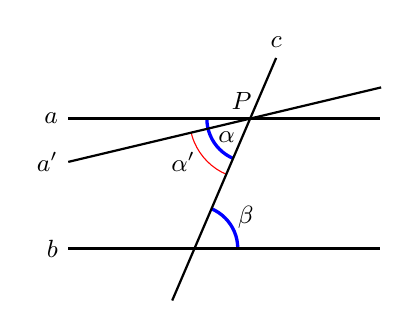
\begin{tikzpicture}[scale=1.1,font=\small, dot/.style={circle,inner sep=1pt, fill, label={#1}, name=#1}, extended line/.style={shorten >=-#1,shorten <=-#1}, extended line/.default=1cm]
\usetikzlibrary{calc, intersections}

\begin{scope}

\coordinate (a1) at (-1.8,0);
\coordinate (a2) at (1.8,0);
\coordinate (b1) at (-1.8,-1.5);
\coordinate (b2) at (1.8,-1.5);

\coordinate (aa1) at (-1.8,-0.5);

\coordinate (c1) at (0.6,0.7);
\coordinate (c2) at (-0.6,-2.1);

\coordinate (p1) at (intersection of c1--c2 and a1--a2);
\coordinate (p2) at (intersection of c1--c2 and b1--b2);


\begin{scope}
\clip (aa1) -- (p1) -- (c2) -- cycle;
\draw[red] (p1) circle (0.7) node[shift={(-0.85,-0.55)}, black] {$\alpha'$};
\end{scope}

\begin{scope}
\clip (a1) -- (p1) -- (c2) -- cycle;
\draw[blue, very thick] (p1) circle (0.5) node[shift={(-0.3,-0.23)}, black] {$\alpha$};
\end{scope}

\begin{scope}
\clip (b2) -- (p2) -- (c1) -- cycle;
\draw[blue, very thick] (p2) circle (0.5) node[shift={(0.65,0.4)}, black] {$\beta$};
\end{scope}


\draw[thick] (a1) node[left] {$a$} --(a2);
\draw[thick] (aa1) node[left] {$a'$} -- ($(aa1)!1.72!(p1)$);
\draw[thick] (b1) node[left] {$b$} --(b2);
\draw[thick] (c1) node[above] {$c$} --(c2);
\node at ([shift={(-0.1,0.2)}]p1) {$P$};

\end{scope}


\end{tikzpicture}

\end{minipage}
~\\

In generale possiamo enunciare il seguente
\begin{teorema}
  Se due rette sono parallele allora esse formano con una trasversale 
  qualunque
  \begin{itemize*}
    \item angoli alterni interni o alterni esterni congruenti;
    \item angoli corrispondenti congruenti;
    \item angoli coniugati interni o coniugati esterni supplementari.
  \end{itemize*}
\end{teorema}

\begin{proof}
  Abbiamo già dimostrato che sono congruenti gli angoli alterni interni 
  formati da due parallele tagliate da una trasversale. Tenendo conto 
  che gli angoli opposti al vertice sono congruenti e gli angoli 
  adiacenti sono supplementari, si possono dedurre facilmente tutte le 
  tesi di questo teorema.
\end{proof}


\section{Somma degli angoli interni di un triangolo}
  \label{sect:angoli_interni_triangolo}

Passiamo ora a dimostrare il secondo teorema dell'angolo esterno di 
un triangolo.
\begin{teorema}
  In un triangolo, un angolo esterno è congruente alla somma dei due 
  angoli interni non adiacenti.
\end{teorema}


\begin{inaccessibleblock}[Figura: TODO]
  \begin{figure}[htb]
    \centering% Copyright (c) 2015 Daniele Masini - d.masini.it@gmail.com

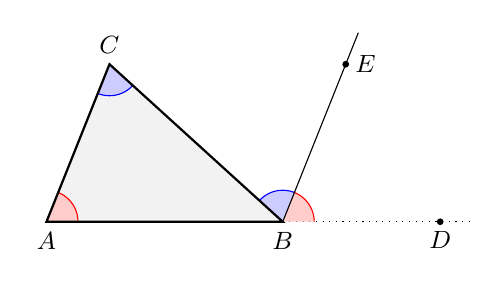
\begin{tikzpicture}[scale=1,font=\small, dot/.style={circle,inner sep=1pt, fill, label={#1}, name=#1}, extended line/.style={shorten >=-#1,shorten <=-#1}, extended line/.default=1cm]
\usetikzlibrary{calc, intersections}

\begin{scope}

\coordinate (a) at (0,0);
\coordinate (b) at (3,0);
\coordinate (c) at (0.8,2);
\coordinate (d) at (5,0);
\coordinate (e) at (3.8,2);

\draw[fill, gray!10] (a) node[below] {$A$} -- (b) node[below] {$B$} -- (c) node[above] {$C$} -- cycle;
\draw[dotted] (b) -- ($(b)!1.2!(d)$);
\draw[fill] (d) circle (1pt) node[below] {$D$};

\begin{scope}
\clip (a) -- (b) -- (c) -- cycle;
\draw[red,fill=red!20] (a) circle (0.4) node[shift={(-0.85,-0.55)}, black] {$\alpha'$};
\draw[blue,fill=blue!20] (c) circle (0.4) node[shift={(-0.85,-0.55)}, black] {$\alpha'$};
\end{scope}

\begin{scope}
\clip (b) -- (e) -- (d) -- cycle;
\draw[red,fill=red!20] (b) circle (0.4) node[shift={(-0.85,-0.55)}, black] {$\alpha'$};
\end{scope}
\begin{scope}
\clip (b) -- (c) -- (e) -- cycle;
\draw[blue,fill=blue!20] (b) circle (0.4) node[shift={(-0.85,-0.55)}, black] {$\alpha'$};
\end{scope}

\draw[fill] (e) circle (1pt) node[right] {$E$};
\draw (b) -- ($(b)!1.2!(e)$);
\draw[thick] (a) node[below] {$A$} -- (b) node[below] {$B$} -- (c) node[above] {$C$} -- cycle;

\end{scope}


\end{tikzpicture}

  \end{figure}
\end{inaccessibleblock}

\begin{proof}
  Sia $ABC$ un triangolo e sia $C\widehat{B}D$ un angolo esterno. 
  Tracciamo la semiretta $BE\parallel AC$ che divide l'angolo 
  $C\widehat{B}D$ in due parti, $C\widehat{B}E$ ed $E\widehat{B}D$. 
  L'angolo $C\widehat{B}E$ risulta congruente all'angolo 
  $A\widehat{C}B$ in quanto i due angoli sono alterni interni rispetto 
  alle rette parallele $AC$ e $BE$ tagliate dalla trasversale $CB$; 
  analogamente l'angolo $E\widehat{B}D$ risulta congruente all'angolo 
  $C\widehat{A}B$ in quanto i due angoli sono corrispondenti rispetto 
  alle rette parallele $AC$ e $BE$ tagliate dalla trasversale $AD$. 
  Dunque $C\widehat{B}D$ è congruente alla somma degli angoli interni 
  di vertici $A$ e $C$.
\end{proof}

\begin{corollario}
  La somma degli angoli interni di un triangolo è congruente ad un 
  angolo piatto.
\end{corollario}
\begin{proof}
  Dalla figura precedente $A\widehat{B}D\cong A\widehat{B}C + 
  C\widehat{B}E + E\widehat{B}D\cong A\widehat{B}C + B\widehat{C}A + 
  C\widehat{A}B$, pertanto la somma degli angoli interni è congruente 
  all'angolo piatto $A\widehat{B}D$.
\end{proof}
\begin{corollario}
  Un triangolo non può avere più di un angolo retto e/o ottuso.
\end{corollario}
Dunque, necessariamente almeno due angoli sono acuti. Di conseguenza, 
gli angoli alla base di un triangolo isoscele devono essere acuti.

\section{Somma degli angoli interni di un poligono}
  \label{sect:angoli_interni_poligono}

\begin{teorema}
  Dato un poligono $P$ di $n$ lati, la somma degli angoli interni di 
  $P$ è $n-2$ angoli piatti.
\end{teorema}
\noindent \begin{minipage}{0.5\textwidth}
  \begin{proof}
    Infatti, dato un qualunque poligono (anche concavo) di $n$ lati, 
    scelto un opportuno punto interno $J$ in modo che, congiunto con esso 
    ciascun vertice il poligono resti diviso in $n$ triangoli, si può 
    osservare che la somma degli angoli interni del poligono è data dalla 
    somma degli angoli interni di $n$ triangoli ($n$ angoli piatti) meno 
    l'angolo giro (2 angoli piatti) in $J$.
  \end{proof}
\end{minipage}\hfil
\begin{minipage}{0.5\textwidth}
  \centering% Copyright (c) 2015 Daniele Masini - d.masini.it@gmail.com

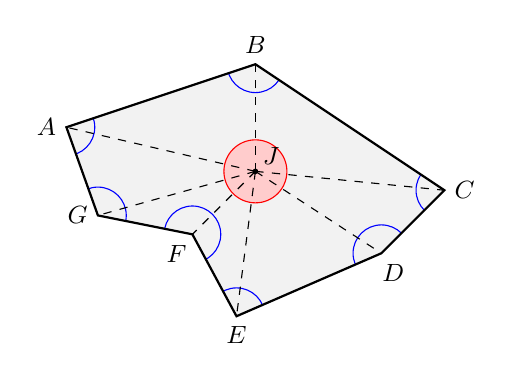
\begin{tikzpicture}[scale=0.8,font=\small, dot/.style={circle,inner sep=1pt, fill, label={#1}, name=#1}, extended line/.style={shorten >=-#1,shorten <=-#1}, extended line/.default=1cm]
\usetikzlibrary{calc, intersections}

\begin{scope}

\coordinate (a) at (0,0);
\coordinate (b) at (3,1);
\coordinate (c) at (6,-1);
\coordinate (d) at (5,-2);
\coordinate (e) at (2.7,-3);
\coordinate (f) at (2,-1.7);
\coordinate (g) at (0.5,-1.4);
\coordinate (j) at (3,-0.7);

\draw[fill, gray!10] (a) -- (b) -- (c) -- (d) -- (e) -- (f) -- (g) -- cycle;
\draw[red, fill=red!20] (j) circle (0.5);

\begin{scope}
\clip (a) -- (b) -- (c) -- (d) -- (e) -- (f) -- (g) -- cycle;
\draw[blue] (a) circle (0.45);
\draw[blue] (b) circle (0.45);
\draw[blue] (c) circle (0.45);
\draw[blue] (d) circle (0.45);
\draw[blue] (e) circle (0.45);
\draw[blue] (f) circle (0.45);
\draw[blue] (g) circle (0.45);
\end{scope}

\draw[fill] (j) circle (1pt) node[shift={(0.2,0.2)}] {$J$};
\draw[dashed] (j) -- (a);
\draw[dashed] (j) -- (b);
\draw[dashed] (j) -- (c);
\draw[dashed] (j) -- (d);
\draw[dashed] (j) -- (e);
\draw[dashed] (j) -- (f);
\draw[dashed] (j) -- (g);

\draw[thick] (a) node[left] {$A$} -- (b) node[above] {$B$} -- (c) node[right] {$C$} -- (d) node[shift={(0.15,-0.25)}] {$D$} -- (e) node[below] {$E$} -- (f) node[shift={(-0.2,-0.25)}] {$F$} -- (g) node[left] {$G$} -- cycle;

\end{scope}


\end{tikzpicture}

\end{minipage}

\begin{teorema}
  La somma degli angoli esterni di un qualsiasi poligono convesso, 
  indipendentemente dal numero dei lati, è congruente ad un angolo giro.
\end{teorema}
\noindent \begin{minipage}{0.5\textwidth}
  \begin{proof}
    Ogni angolo esterno è adiacente ad un angolo interno, per cui se si 
    hanno $m$ lati, e quindi $m$ vertici, la somma degli angoli interni e 
    degli angoli esterni è pari ad $m$ angoli piatti. Essendo la somma 
    degli angoli interni congruente a $m-2$ angoli piatti (per il teorema 
    precedente), la somma degli angoli esterni sarà di due angoli piatti, 
    cioè un angolo giro.
  \end{proof}
\end{minipage}\hfil
\begin{minipage}{0.5\textwidth}
  \centering% Copyright (c) 2015 Daniele Masini - d.masini.it@gmail.com

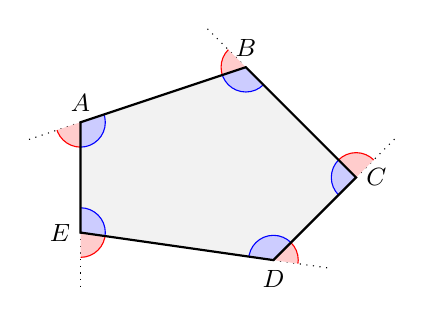
\begin{tikzpicture}[scale=0.7,font=\small, dot/.style={circle,inner sep=1pt, fill, label={#1}, name=#1}, extended line/.style={shorten >=-#1,shorten <=-#1}, extended line/.default=1cm]
\usetikzlibrary{calc, intersections}

\begin{scope}

\coordinate (a) at (0,0);
\coordinate (b) at (3,1);
\coordinate (c) at (5,-1);
\coordinate (d) at (3.5,-2.5);
\coordinate (e) at (0,-2);
\coordinate (f) at (2.4,-0.7);

\draw[fill, gray!10] (a) -- (b) -- (c) -- (d) -- (e) -- cycle;
%\draw[red, fill=red!20] (f) circle (0.5);

\begin{scope}
\clip (a) -- (b) -- (c) -- (d) -- (e) -- cycle;
\draw[blue, fill=blue!20] (a) circle (0.45);
\draw[blue, fill=blue!20] (b) circle (0.45);
\draw[blue, fill=blue!20] (c) circle (0.45);
\draw[blue, fill=blue!20] (d) circle (0.45);
\draw[blue, fill=blue!20] (e) circle (0.45);
\end{scope}

\draw[dotted] (a) -- ($(a)!-1cm!(b)$) coordinate (a1);
\draw[dotted] (b) -- ($(b)!-1cm!(c)$) coordinate (b1);
\draw[dotted] (c) -- ($(c)!-1cm!(d)$) coordinate (c1);
\draw[dotted] (d) -- ($(d)!-1cm!(e)$) coordinate (d1);
\draw[dotted] (e) -- ($(e)!-1cm!(a)$) coordinate (e1);

\begin{scope}
\clip (a) -- (e) -- (a1) -- cycle;
\draw[red, fill=red!20] (a) circle (0.45);
\end{scope}
\begin{scope}
\clip (b) -- (a) -- (b1) -- cycle;
\draw[red, fill=red!20] (b) circle (0.45);
\end{scope}
\begin{scope}
\clip (c) -- (b) -- (c1) -- cycle;
\draw[red, fill=red!20] (c) circle (0.45);
\end{scope}
\begin{scope}
\clip (d) -- (c) -- (d1) -- cycle;
\draw[red, fill=red!20] (d) circle (0.45);
\end{scope}
\begin{scope}
\clip (e) -- (d) -- (e1) -- cycle;
\draw[red, fill=red!20] (e) circle (0.45);
\end{scope}

%\draw[fill] (f) circle (1pt) node[below] {$F$};
%\draw[dashed] (f) -- (a);
%\draw[dashed] (f) -- (b);
%\draw[dashed] (f) -- (c);
%\draw[dashed] (f) -- (d);
%\draw[dashed] (f) -- (e);

\draw[thick] (a) node[above] {$A$} -- (b) node[above] {$B$} -- (c) node[right] {$C$} -- (d) node[below] {$D$} -- (e) node[left] {$E$} -- cycle;

\end{scope}


\end{tikzpicture}

\end{minipage}


\section{Generalizzazione dei criteri di congruenza dei 
  triangoli}\label{sect:generalizzazione_criteri_congruenza_triangoli}

Se due triangoli hanno rispettivamente due angoli congruenti, allora 
anche i terzi angoli saranno congruenti nei due triangoli, in quanto 
supplementari della somma di angoli congruenti.

Dunque, se due triangoli hanno congruenti un lato e due angoli, anche 
se il lato congruente non è compreso tra i due angoli congruenti, 
risultano congruenti. Precisamente, vale la seguente proposizione.

\begin{teorema}[Generalizzazione del 2\textsuperscript{o} criterio di 
  congruenza dei triangoli]
  Due triangoli sono congruenti se hanno rispettivamente congruenti una 
  coppia di lati e due coppie di angoli ugualmente posti rispetto ai 
  lati congruenti.
\end{teorema}


\begin{inaccessibleblock}[Figura: TODO]
  \begin{figure}[htb]
    \centering% Copyright (c) 2015 Daniele Masini - d.masini.it@gmail.com

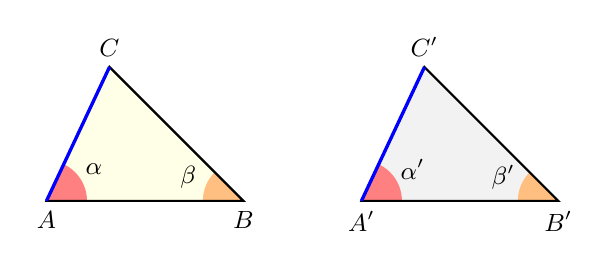
\begin{tikzpicture}[scale=1,font=\small]
\usetikzlibrary{calc}

\begin{scope}
\coordinate (a) at (0,0);
\coordinate (c) at (0.8,1.7);
\coordinate (b) at (2.5,0);
\draw[fill=yellow!10] (a) -- (b) -- (c) -- cycle;

\begin{scope}
\clip (a) -- (b) -- (c) -- cycle;
\draw[thick,red!50,fill] (a) circle (0.5);
\node at ([shift={(0.6,0.4)}]a) {$\alpha$};
\draw[thick,orange!50,fill] (b) circle (0.5);
\node at ([shift={(-0.7,0.3)}]b) {$\beta$};
\end{scope}

\draw[thick] (a) node[below] {$A$} -- (b) node[below] {$B$} -- (c) node[above] {$C$} -- cycle;
\draw[blue,very thick] (a) -- (c);


\end{scope}

\begin{scope}[xshift=4cm]
\coordinate (a) at (0,0);
\coordinate (c) at (0.8,1.7);
\coordinate (b) at (2.5,0);
\draw[fill=gray!10] (a) -- (b) -- (c) -- cycle;

\begin{scope}
\clip (a) -- (b) -- (c) -- cycle;
\draw[thick,red!50,fill] (a) circle (0.5);
\node at ([shift={(0.65,0.4)}]a) {$\alpha'$};
\draw[thick,orange!50,fill] (b) circle (0.5);
\node at ([shift={(-0.7,0.3)}]b) {$\beta'$};
\end{scope}

\draw[thick] (a) node[below] {$A'$} -- (b) node[below] {$B'$} -- (c) node[above] {$C'$} -- cycle;
\draw[blue,very thick] (a) -- (c);

\end{scope}

\end{tikzpicture}

  \end{figure}
\end{inaccessibleblock}

\begin{proof}
  Il caso in cui il lato congruente è compreso tra gli angoli 
  congruenti è stato già dimostrato (2\textsuperscript{o} criterio di 
  congruenza dei triangoli) ed utilizzato per la dimostrazione di varie 
  proprietà. Ora consideriamo l'altro caso.
  
  In figura abbiamo rappresentato due triangoli, $ABC$ e $A'B'C'$ che 
  hanno per ipotesi i lati $AC\cong A'C'$ e gli angoli $\alpha\cong 
  \alpha'$ e $\beta\cong \beta'$. I due triangoli risultano congruenti, 
  poiché deve risultare $A\widehat{C}B\cong A'\widehat{C'}B'$, in 
  quanto tali angoli sono supplementari alla somma di angoli congruenti 
  per ipotesi (la somma degli angoli interni di un triangolo è un 
  angolo piatto). Ci riconduciamo quindi al caso del 
  2\textsuperscript{o} criterio di congruenza, già dimostrato in 
  precedenza.
\end{proof}

Riprendiamo una proprietà dei triangoli isosceli che abbiamo 
enunciato ma non abbiamo dimostrato.
\begin{proposizione}
  In un triangolo isoscele, l'altezza relativa alla base è anche 
  bisettrice dell'angolo al vertice e mediana relativa alla base.
\end{proposizione}

\noindent \begin{minipage}{0.6\textwidth}
  \noindent Ipotesi: $IG\cong IH$, $\alpha\cong \beta$, $IL\perp GH$.\\
  Tesi: $G\widehat{I}L\cong H\widehat{I}L$, $GL\cong LH$.
  
  \begin{proof}
    I triangoli $GLI$ e $LHI$ sono congruenti per il secondo criterio 
    generalizzato, avendo congruenti un lato (quello obliquo, $IG\cong 
    IH$) e due angoli ($\alpha\cong \beta$ e $I\widehat{L}G \cong 
    I\widehat{L}H$). Di conseguenza, i restanti elementi sono 
    ordinatamente congruenti, in particolare $GL\cong LH$ e 
    $G\widehat{I}L\cong H\widehat{I}L$.
  \end{proof}
\end{minipage}\hfil
\begin{minipage}{0.4\textwidth}
  \centering% Copyright (c) 2015 Daniele Masini - d.masini.it@gmail.com

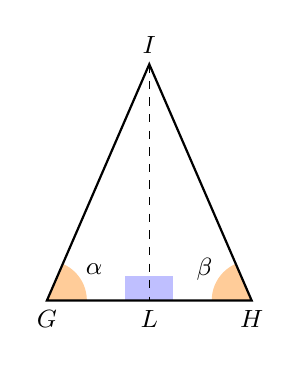
\begin{tikzpicture}[scale=1,font=\small]
\usetikzlibrary{calc}

\begin{scope}
\coordinate (a) at (-1.3,0);
\coordinate (b) at (1.3,0);
\coordinate (c) at (0,3);
\coordinate (j) at (0,0);

\begin{scope}
\clip (a) -- (b) -- (c) -- cycle;
\draw[fill,orange!40] (a) circle (0.5);
\draw[fill,orange!40] (b) circle (0.5);
\node at ([shift={(0.6,0.4)}]a) {$\alpha$};
\node at ([shift={(-0.6,0.4)}]b) {$\beta$};
\coordinate (j1) at ($(j)!0.3cm!(b)$);
\draw[fill,blue!25] ($(j)!0.3cm!(a)$) rectangle ($(j1)!0.3cm!90:(b)$);
\end{scope}

\draw[dashed] (c) -- (j) node[below] {$L$};
\draw[thick] (a) node[below] {$G$} -- (b) node[below] {$H$} -- (c) node[above] {$I$} -- cycle;

\end{scope}

\end{tikzpicture}

\end{minipage}

\osservazione Dall'esame dei primi tre criteri di congruenza dei 
triangoli, nonché dalla generalizzazione del secondo criterio, si 
potrebbe essere indotti a pensare che due triangoli sono congruenti 
se hanno tre coppie di elementi rispettivamente congruenti, se almeno 
una delle tre coppie di elementi è costituita da lati.

\noindent \begin{minipage}{0.6\textwidth}
  In realtà, il primo criterio non si può generalizzare come il 
  secondo. Basta pensare alla figura a lato: $ADC$ è un triangolo 
  isoscele, $B$ è un punto sul prolungamento della base $AD$. Unendo $B$ 
  con $C$, vengono individuati due nuovi triangoli, $ABC$ e $BCD$ che 
  hanno in comune il lato $CB$ e l'angolo di vertice $B$, ed hanno 
  inoltre congruenti i lati $AC$ e $CD$, ma evidentemente non sono 
  congruenti. Quindi se due triangoli hanno due lati ed un angolo 
  qualsiasi congruenti, non è detto che siano congruenti. Però nei due 
  triangoli citati in figura, gli angoli $C\widehat{A}B$ e 
  $C\widehat{D}B$ sono supplementari.
\end{minipage}\hfil
\begin{minipage}{0.4\textwidth}
  \centering% Copyright (c) 2015 Daniele Masini - d.masini.it@gmail.com

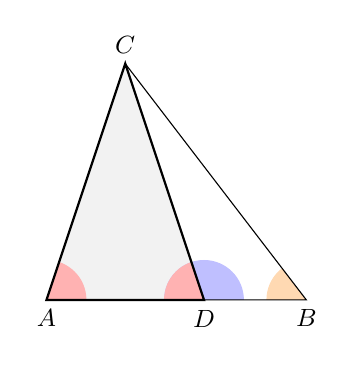
\begin{tikzpicture}[scale=1,font=\small]
\usetikzlibrary{calc}

\begin{scope}
\coordinate (a) at (-1,0);
\coordinate (b) at (2.3,0);
\coordinate (c) at (0,3);
\coordinate (d) at (1,0);

\coordinate (j) at (0,0);

\draw[fill, gray!10] (a) -- (d) -- (c) -- cycle;

\begin{scope}
\clip (a) -- (b) -- (c) -- cycle;
\draw[fill,red!30] (a) circle (0.5);
\draw[fill,orange!30] (b) circle (0.5);
%\node at ([shift={(0.6,0.4)}]a) {$\alpha$};
%\node at ([shift={(-0.6,0.4)}]b) {$\beta$};
\draw[fill,blue!25] (d) circle (0.5);
\end{scope}

\begin{scope}
\clip (a) -- (d) -- (c) -- cycle;
\draw[fill,red!30] (d) circle (0.5);
\end{scope}

\draw[thick] (a) -- (c) -- (d) node[below] {$D$} -- cycle;
\draw (a) node[below] {$A$} -- (b) node[below] {$B$} -- (c) node[above] {$C$} -- cycle;

\end{scope}

\end{tikzpicture}

\end{minipage}


\subsection{Congruenze di triangoli rettangoli}

Per quanto affermato nelle proposizioni precedenti, sappiamo che i 
triangoli rettangoli hanno una coppia di angoli congruenti (quelli 
retti, essendo tutti congruenti fra loro, come affermato dal IV 
postulato di Euclide) e gli altri angoli necessariamente acuti, in 
quanto la somma degli angoli interni di un triangolo è congruente ad 
un angolo piatto (come segue dal secondo teorema dell'angolo esterno 
e dai corollari).

Tenendo conto dunque dei criteri di congruenza dei triangoli, si 
possono riformulare dei criteri di congruenza specifici per i 
triangoli rettangoli. Di questi ultimi omettiamo la dimostrazione. 

\begin{teorema}[Criteri di congruenza dei triangoli rettangoli]
  Due triangoli rettangoli sono congruenti se hanno rispettivamente 
  congruenti almeno uno tra:
  \begin{itemize*}
    \item i due cateti (1\textsuperscript{o} criterio);
    \item l'ipotenusa e un angolo acuto (2\textsuperscript{o} criterio);
    \item un cateto e l'angolo acuto adiacente (2\textsuperscript{o} 
    criterio);
    \item un cateto e l'angolo acuto opposto (2\textsuperscript{o} 
    criterio);
    \item un cateto e l'ipotenusa (4\textsuperscript{o} criterio).
  \end{itemize*}
\end{teorema}

A titolo esemplificativo, ecome applicazione dei criteri, proponiamo qui di 
seguito  due possibili costruzioni di triangoli rettangoli mediante l'utilizzo 
della riga e del compasso.

\begin{procedura}
  Costruisci un triangolo rettangolo i cui cateti sono congruenti a due 
segmenti dati:
  \begin{enumerate} [nosep]
    \item 
    Traccia un segmento e denominalo AB.
    \item 
    Traccia un segmento e denominalo CD.
    \item 
    Traccia un punto E e la circonferenza c' di centro E e raggio AB.
    \item 
    Considera sulla circonferenza c' un punto e denominalo F.
    \item 
    Traccia il segmento EF.
    \item 
    Costruisci la retta r passante per E e perpendicolare a EF.
    \item 
    Traccia la circonferenza c'' di centro E e raggio CD.
    \item 
    Denomina G e G' le intersezioni della retta r con la circonferenza c'' 
tracciata.
    \item 
    Il triangolo EFG è rettangolo e ha i due cateti EF e EG congruenti ai due 
segmenti AB e CD dati. 
    \item 
  \end{enumerate}
  Anche il triangolo EFG' è rettangolo e ha i due cateti EF e EG' congruenti ai 
due segmenti AB e CD dati. \end{procedura}

\begin{procedura}
  Costruisci un triangolo rettangolo, dato un cateto e un angolo adiacente al 
cateto:
  \begin{enumerate} [nosep]
    \item 
    Traccia il segmento AB.
    \item 
    Costruisci l'angolo CDE.
    \item 
    Traccia un punto F .
    \item 
    Traccia la circonferenza di centro F e raggio AB.
    \item 
    Traccia arbitrariamente sulla circonferenza un punto G.
    \item 
    Traccia la semiretta di origine G e passante per F.
    \item 
    Trasporta l'angolo CDE sulla semiretta GF.
    \item 
    Costruisci la perpendicolare s a FG e passante per F.
    \item 
    H è il punto di intersezione del secondo lato dell'angolo (diverso dalla 
semiretta FG) con la perpendicolare s.
    \item 
    Il triangolo GFH è il triangolo rettangolo in F, con un angolo acuto 
congruente a CDE (quale?.................) e un cateto congruente ad AB (quale? 
…..............)
  \end{enumerate}
\end{procedura}

\begin{procedura}
  Costruisci un triangolo rettangolo, dato un cateto e l'ipotenusa:
  \begin{enumerate} [nosep]
    \item 
    Traccia un segmento AB e un segmento DE > AB.
    \item 
    Traccia un punto F del piano.
    \item 
    Traccia la circonferenza di centro F e raggio congruente ad AB.
    \item 
    Sia G un punto della circonferenza.
    \item 
    Traccia il segmento FG e la retta r perpendicolare a FG e passante per F.
    \item 
    Traccia la circonferenza di centro G e raggio congruente a DE,
    \item 
    Denomina H il punto di intersezione fra la retta r e la circonferenza.
    \item 
    Il triangolo HFG è il triangolo rettangolo con un cateto congruente ad AB e 
l'ipotenusa congruente a DE.
  \end{enumerate}
  \textsl{Si può dire che il triangolo rettangolo si forma in ogni caso?}
\end{procedura}

\section{Disuguaglianze tra gli elementi di un 
  triangolo}\label{sect:disuguaglianze_triangoli}

\begin{teorema}
  In un triangolo, a lato maggiore si oppone angolo maggiore.
\end{teorema}

\noindent\begin{minipage}{0.7\textwidth}
  \noindent Ipotesi: $BC>AB$. Tesi: $B\widehat{A}C>A\widehat{C}B$.
  
  \begin{proof}
    Scegliamo opportunamente un punto $D$ sul lato maggiore $BC$ in modo 
    che $BD$ sia congruente ad $AB$. Se uniamo $A$ con $D$, poiché il 
    segmento $AD$ è interno al triangolo $ABC$, il triangolo $ABC$ viene 
    diviso in due nuovi triangoli, $ADB$ e $ACD$. Il triangolo $ADB$ è 
    isoscele sulla base $AD$ pertanto ha gli angoli alla base congruenti, 
    per cui risulta $B\widehat{A}D\cong A\widehat{D}B$. Ma 
    $B\widehat{A}D$ è una parte propria di $B\widehat{A}C$, mentre 
    $A\widehat{D}B$, come angolo esterno al triangolo $ACD$ è maggiore 
    dell'angolo $A\widehat{C}D=A\widehat{C}B$, interno non adiacente, per 
    il primo teorema dell'angolo esterno. Si ha dunque: 
    $B\widehat{A}C>B\widehat{A}D\cong A\widehat{D}B>A\widehat{C}B$ e 
    quindi la tesi (in maniera del tutto analoga si può dimostrare che 
    $B\widehat{A}C>A\widehat{B}C$).
  \end{proof}
\end{minipage}\hfil
\begin{minipage}{0.3\textwidth}
  \centering% Copyright (c) 2015 Daniele Masini - d.masini.it@gmail.com

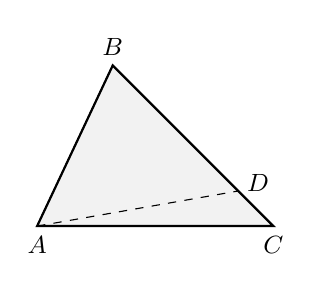
\begin{tikzpicture}[scale=1.2,font=\small]
\usetikzlibrary{calc, through, intersections}

\begin{scope}
\clip (-0.1,-0.5) rectangle (2.6,2.1);
\coordinate (a) at (0,0);
\coordinate (b) at (0.8,1.7);
\coordinate (c) at (2.5,0);
\draw[fill=gray!10] (a) -- (b) -- (c) -- cycle;

\node (c1) at (b) [circle through={(a)}] {};
\coordinate(d) at (intersection 1 of c1 and b--c);

\draw[dashed] (a) -- (d) node[shift={(0.25,0.1)}] {$D$};

\draw[thick] (a) node[below] {$A$} -- (b) node[above] {$B$} -- (c) node[below] {$C$} -- cycle;

\end{scope}

\end{tikzpicture}

\end{minipage}

\begin{teorema}
  In un triangolo, ad angolo maggiore si oppone lato maggiore.
\end{teorema}

\noindent\begin{minipage}{0.7\textwidth}\parindent15pt 
  \noindent Ipotesi: $B\widehat{A}C>A\widehat{C}B$. Tesi: $BC>AB$.
  
  \noindent\begin{proof}
    \noindent Dimostriamo la tesi in maniera indiretta, facendo uso del 
    teorema precedente e del teorema del triangolo isoscele. Supponiamo 
    vera l'ipotesi $B\widehat{A}C>A\widehat{C}B$. Facciamo un confronto 
    tra i segmenti $BC$ e $AB$ considerando tutte le possibilità. \`E 
    possibile che sia:
    \[\text{(i) }BC\cong AB\text{;}\qquad\qquad \text{(ii) 
    }BC<AB\text{;}\quad\quad\text{(iii) }BC>AB\text{.}\]
    
    Se fosse vera la (i), il triangolo $ABC$ sarebbe isoscele sulla base 
    $AC$ e risulterebbe $B\widehat{A}C\cong A\widehat{C}B$, per il 
    teorema del triangolo isoscele, contro l'ipotesi.
    
    Se fosse vera la (ii), per il teorema precedente risulterebbe 
    $B\widehat{A}C<A\widehat{C}B$, contro l'ipotesi.
    
    Rimane solo la possibilità che sia vera la (iii), la quale infatti 
    non contraddice il teorema precedente, anzi lo conferma. Quindi la 
    tesi è dimostrata.
  \end{proof}
\end{minipage}\hfil
\begin{minipage}{0.3\textwidth}
  \centering% Copyright (c) 2015 Daniele Masini - d.masini.it@gmail.com

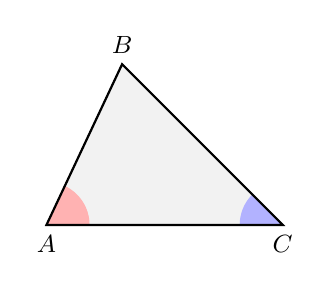
\begin{tikzpicture}[scale=1.2,font=\small]
\usetikzlibrary{calc, through, intersections}

\begin{scope}
\coordinate (a) at (0,0);
\coordinate (b) at (0.8,1.7);
\coordinate (c) at (2.5,0);
\draw[fill=gray!10] (a) -- (b) -- (c) -- cycle;

\begin{scope}
\clip (a) -- (b) -- (c);
\draw[fill, red!30] (a) circle (0.45);
\draw[fill, blue!30] (c) circle (0.45);
\end{scope}

\draw[thick] (a) node[below] {$A$} -- (b) node[above] {$B$} -- (c) node[below] {$C$} -- cycle;

\end{scope}

\end{tikzpicture}

\end{minipage}
~\\

Da questo teorema discende la proprietà che in un triangolo 
rettangolo l'ipotenusa è sempre maggiore di ciascuno dei due cateti, 
in quanto l'ipotenusa è il lato che si oppone all'angolo maggiore, 
l'angolo retto.

Ora dimostriamo una proprietà importante dei triangoli, nota come 
\emph{disuguaglianza triangolare}.

\begin{teorema}[Disuguaglianza triangolare]
  In un triangolo, ciascun lato è minore della somma degli altri due e 
  maggiore della loro differenza.
\end{teorema}

  \begin{proof}
~

\noindent\begin{minipage}{0.7\textwidth}\parindent15pt 
    In riferimento alla figura a lato, dimostriamo che nel triangolo 
    $ABC$, $AC < AB + BC$. Se $AC$ fosse minore di un altro lato, 
    sicuramente sarebbe minore della somma degli altri due e il teorema 
    sarebbe dimostrato. Esaminiamo il caso in cui $AC$ è maggiore sia di 
    $AB$ che di $BC$. Prolunghiamo il lato $AB$ dalla parte di $B$ e 
    prendiamo un punto $D$ sul prolungamento in modo che il segmento $BD$ 
    sia congruente a $BC$. Unendo $D$ con $C$ abbiamo il triangolo $ACD$ 
    nel quale il lato $AD$ è congruente alla somma dei lati $AB$ e $BC$. 
    La tesi si riconduce dunque a dimostrare che il lato $AC$ è minore di 
    $AD$. Osserviamo che il triangolo $CBD$ è isoscele sulla base $CD$, 
    per cui i suoi angoli alla base sono congruenti: $B\widehat{C}D\cong 
    B\widehat{D}C$. Ma l'angolo $B\widehat{C}D$ è una parte propria di 
    $A\widehat{C}D$ che quindi risulta maggiore di $B\widehat{C}D\cong 
    A\widehat{D}C$. Dunque, nel triangolo $ACD$, il lato $AD$, che si 
    oppone ad angolo maggiore, è maggiore del lato $AC$, che si oppone ad 
    angolo minore, per il teorema precedente.
\end{minipage}\hfil
\begin{minipage}{0.3\textwidth}
  \centering% Copyright (c) 2015 Daniele Masini - d.masini.it@gmail.com

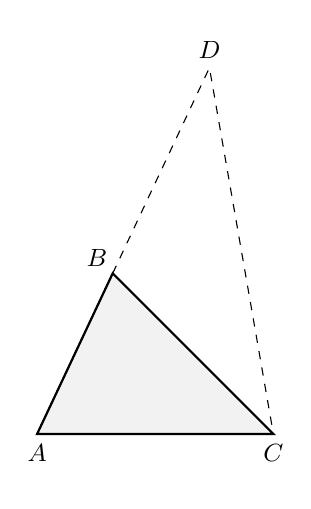
\begin{tikzpicture}[scale=1.2,font=\small]
\usetikzlibrary{calc, through, intersections}

\begin{scope}
\clip (-0.1,-0.5) rectangle (2.6,4.3);
\coordinate (a) at (0,0);
\coordinate (b) at (0.8,1.7);
\coordinate (c) at (2.5,0);
\draw[fill=gray!10] (a) -- (b) -- (c) -- cycle;

\node (c1) at (b) [circle through={(c)}] {};
\coordinate(d) at (intersection 1 of c1 and a--b);

\draw[dashed] (b) -- (d) node[above] {$D$} -- (c);

\draw[thick] (a) node[below] {$A$} -- (b) node[shift={(-0.2,0.2)}] {$B$} -- (c) node[below] {$C$} -- cycle;

\end{scope}

\end{tikzpicture}

\end{minipage}
    
    Visto che la costruzione fatta si può ripetere tale e quale rispetto 
    a qualsiasi lato, si può concludere che $AC<AB+BC$, $AB<AC+BC$, 
    $BC<AB+AC$ e dunque, sottraendo ad ambo i membri della prima 
    disuguaglianza il lato $BC$ si ha $AC-AB<BC$, analogamente, 
    sottraendo uno stesso segmento, si hanno $AC-BC<AB$, $AC-BC<AB$, 
    $AB-AC<BC$, $AB-BC<AC$, $BC-AC<AB$, $BC-AB<AC$. Leggendo le relazioni 
    da destra verso sinistra, ogni lato è maggiore della differenza degli 
    altri due (abbiamo scritto tutte le disuguaglianze, anche se 
    ovviamente ogni lato ha misura positiva mentre la differenza tra due 
    lati può essere anche nulla o negativa).
  \end{proof}

Proponiamo ora un teorema sulle disuguaglianze tra gli elementi di 
due triangoli.

Supponiamo di avere due triangoli aventi due coppie di lati 
rispettivamente congruenti. Allora, se anche gli angoli compresi sono 
congruenti, i due triangoli risultano congruenti per il primo 
criterio. Altrimenti, se i due angoli compresi tra i lati congruenti 
non sono congruenti, i due triangoli non sono congruenti, ed i terzi 
lati sono diseguali nello stesso verso degli angoli opposti ad essi 
(cioè compresi tra i lati congruenti).

\begin{teorema}
  Se due lati di un triangolo sono rispettivamente congruenti a due 
  lati di un altro triangolo, e l'angolo tra essi compreso è nel primo 
  triangolo maggiore che nel secondo, allora il terzo lato del primo 
  triangolo è maggiore del terzo lato del secondo.
\end{teorema}

\noindent Ipotesi: $AB\cong DE$, $AC\cong DF$, 
$B\widehat{A}C>E\widehat{D}F$ ($AB\leq AC$). Tesi: $BC>EF$.


\begin{inaccessibleblock}[Figura: TODO]
  \begin{figure}[htb]
    \centering% Copyright (c) 2015 Daniele Masini - d.masini.it@gmail.com

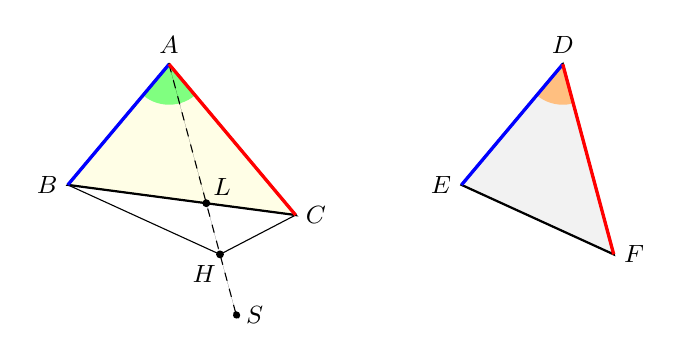
\begin{tikzpicture}[scale=1,font=\small]
\usetikzlibrary{calc}

\begin{scope}

\draw[fill=yellow!10] (0,0) coordinate (b) -- ++(50:2) coordinate (a) -- ++(-50:2.5) coordinate (c) -- cycle;

\begin{scope}
\clip (a) -- (b) -- (c) -- cycle;
\draw[thick,green!50,fill] (a) circle (0.5);
%\node at ([shift={(0.65,0.4)}]a) {$\beta$};
\end{scope}

\draw[fill,dashed] (a) -- ++(-75:3.3) circle (1.2pt) coordinate (s) node[right] {$S$};
\draw[fill] ($(a)!{2.5/3.3}!(s)$) circle (1.2pt) coordinate (h) node[shift={(-0.2,-0.25)}] {$H$};
\draw (h) -- (b);

\coordinate (l) at (intersection of a--s and b--c);
\draw[fill] (l) circle (1.2pt) node[shift={(0.2,0.2)}] {$L$};
\draw (h) -- (c);

\draw[thick] (a) node[above] {$A$} -- (b) node[left] {$B$} -- (c) node[right] {$C$} -- cycle;
\draw[blue,very thick] (a) -- (b);
\draw[red,very thick] (a) -- (c);

\end{scope}

\begin{scope}[xshift=5cm]

\draw[fill=gray!10] (0,0) coordinate (b) -- ++(50:2) coordinate (a) -- ++(-75:2.5) coordinate (c) -- cycle;

\begin{scope}
\clip (a) -- (b) -- (c) -- cycle;
\draw[thick,orange!50,fill] (a) circle (0.5);
%\node at ([shift={(0.65,0.4)}]a) {$\beta$};
\end{scope}

\draw[thick] (a) node[above] {$D$} -- (b) node[left] {$E$} -- (c) node[right] {$F$} -- cycle;
\draw[blue,very thick] (a) -- (b);
\draw[red,very thick] (a) -- (c);

\end{scope}

\end{tikzpicture}

  \end{figure}
\end{inaccessibleblock}

\begin{proof}
  Tracciamo la semiretta $AS$ di origine $A$, interna all'angolo 
  $B\widehat{A}C$, in modo tale che $B\widehat{A}S\cong E\widehat{D}F$. 
  Se prendiamo su $AS$ il punto $H$ tale che $AH\cong DF$ ed uniamo $H$ 
  con $B$, otteniamo un triangolo $ABH$ congruente a $DEF$ per il primo 
  criterio.
  
  \`E importante dimostrare che il punto $H$ è esterno al triangolo 
  $ABC$. Per dimostrare ciò, prendiamo il punto $L$, intersezione tra 
  la semiretta $AS$ ed il lato $BC$. Notiamo che abbiamo iniziato la 
  costruzione a partire dal lato $AB$ avendo supposto $AB\leq AC$, ma 
  da questa disuguaglianza segue la corrispondente disuguaglianza tra 
  gli angoli opposti: $A\widehat{B}C\geq A\widehat{C}B$. L'angolo 
  $A\widehat{L}C$ è esterno al triangolo $ABL$, pertanto è maggiore 
  dell'angolo $A\widehat{B}C$ per il primo teorema dell'angolo esterno. 
  Mettendo insieme le due disuguaglianze si ha 
  $A\widehat{L}C>A\widehat{B}C\geq A\widehat{C}B$, dunque nel triangolo 
  $ALC$ vale la seguente relazione tra due angoli: 
  $A\widehat{L}C>A\widehat{C}B$. Vale quindi anche la corrispondente 
  relazione tra i lati opposti, per cui $AC>AL$. Poiché $AX\cong 
  DF\cong AC$, il punto $L$ è interno al segmento $AH$, e dunque $H$ è 
  esterno al triangolo $ABC$.
  
  Abbiamo già unito $H$ con $B$, uniamo $H$ anche con $C$ e ragioniamo 
  sul triangolo $BHC$. Essendo $BH$ congruente ad $EF$, la tesi è 
  ricondotta a dimostrare che $BC$ è maggiore di $BH$. Confrontiamo i 
  rispettivi angoli opposti. Poiché il triangolo $AHC$ è isoscele sulla 
  base $HC$, gli angoli alla base risultano congruenti 
  $A\widehat{H}C\cong A\widehat{C}H$, dunque risulta 
  $B\widehat{H}C\cong B\widehat{C}H$ perché:
  \[B\widehat{H}C=B\widehat{H}A+A\widehat{H}C>A\widehat{H}C\cong 
  A\widehat{C}H=A\widehat{C}B+B\widehat{C}H>B\widehat{C}H.\]
  Dalla precedente disuguaglianza tra gli angoli segue la 
  corrispondente disuguaglianza tra i lati opposti $BC>BH$ e dunque la 
  tesi.
\end{proof}

\begin{teorema}
  Se due lati di un triangolo sono, rispettivamente, congruenti a due 
  lati di un altro triangolo, e il terzo lato del primo triangolo è 
  maggiore del terzo lato del secondo, allora l'angolo opposto al lato 
  diseguale (compreso tra i lati congruenti) è nel primo triangolo 
  maggiore che nel secondo.
\end{teorema}

\noindent Ipotesi: $AB\cong DE$, $AC\cong DF$, $BC>EF$. Tesi: 
$B\widehat{A}C>E\widehat{D}F$.


\begin{inaccessibleblock}[Figura: TODO]
  \begin{figure}[htb]
    \centering% Copyright (c) 2015 Daniele Masini - d.masini.it@gmail.com

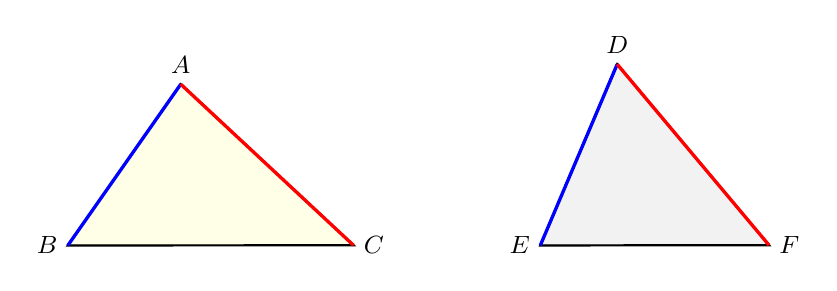
\begin{tikzpicture}[scale=1,font=\small]
\usetikzlibrary{calc}

\begin{scope}

\draw[fill=yellow!10] (0,0) coordinate (b) -- ++(55:2.5) coordinate (a) -- ++(-43:3) coordinate (c) -- cycle;

\draw[thick] (a) node[above] {$A$} -- (b) node[left] {$B$} -- (c) node[right] {$C$} -- cycle;
\draw[blue,very thick] (a) -- (b);
\draw[red,very thick] (a) -- (c);

\end{scope}

\begin{scope}[xshift=6cm]

\draw[fill=gray!10] (0,0) coordinate (b) -- ++(67:2.5) coordinate (a) -- ++(-50:3) coordinate (c) -- cycle;

\draw[thick] (a) node[above] {$D$} -- (b) node[left] {$E$} -- (c) node[right] {$F$} -- cycle;
\draw[blue,very thick] (a) -- (b);
\draw[red,very thick] (a) -- (c);

\end{scope}

\end{tikzpicture}

  \end{figure}
\end{inaccessibleblock}

\begin{proof}
  Procediamo per esclusione, in maniera analoga a come abbiamo fatto 
  nel teorema inverso sulle disuguaglianze tra gli elementi di un 
  triangolo.
  
  Supponiamo vera l'ipotesi e studiamo i vari casi delle possibili 
  relazioni tra gli angoli citati nella tesi. Sono possibili tre casi:
  \[\text{(i) }B\widehat{A}C\cong E\widehat{D}F\text{;}\qquad\qquad 
  \text{(ii) }B\widehat{A}C<E\widehat{D}F\text{;}\qquad\qquad 
  \text{(iii) }B\widehat{A}C>E\widehat{D}F\text{.}\]
  
  Se valesse l'ipotesi (i), essendo anche $AB\cong DE$ e $AC\cong DF$, 
  i triangoli risulterebbero congruenti per il primo criterio, 
  contrariamente all'ipotesi $BC>EF$.
  
  Se valesse l'ipotesi (ii), essendo anche $AB\cong DE$ e $AC\cong DF$, 
  per il teorema precedente risulterebbe $BC<EF$, contrariamente 
  all'ipotesi $BC>EF$.
  
  Rimane l'ipotesi (iii), che non contraddice il teorema precedente e 
  che anzi lo conferma. Dunque la tesi è dimostrata.
\end{proof}


\begin{exrig}
  \begin{esempio}
    Nel triangolo $ABC$, isoscele sulla base $BC$, sia $D$ un punto 
    qualsiasi sul lato $AB$. Dimostra che $DC>DB$.
    
    \noindent\begin{minipage}{0.7\textwidth}\parindent15pt
      \vspace{10pt}
      \noindent Individuiamo ipotesi, tesi e costruiamo il 
      disegno.\vspace{7pt}
      
      \noindent Ipotesi: $AB\cong AC$, $D\in AB$.\tab Tesi: $CD>BD$.
      
      \noindent\begin{proof}
        Consideriamo i triangoli $ABC$ e $DBC$ a lato.\\
        Poiché $B\widehat{C}D<B\widehat{C}A$ e $B\widehat{C}A\cong 
        A\widehat{B}C$ si ha che $B\widehat{C}D<D\widehat{B}C$.
        Quindi, poiché in un triangolo ad angolo maggiore si oppone lato 
        maggiore, considerando il triangolo $DBC$ si ha $CD>BD$.
      \end{proof}
    \end{minipage}\hfil
    \begin{minipage}{0.3\textwidth}
      \centering% Copyright (c) 2015 Daniele Masini - d.masini.it@gmail.com

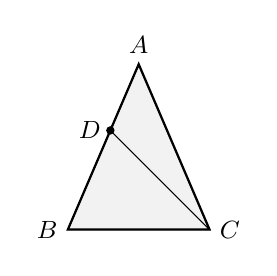
\begin{tikzpicture}[scale=1,font=\small]
\usetikzlibrary{calc, through, intersections}

\begin{scope}
\coordinate (a) at (0,0);
\coordinate (b) at (-0.9,-2.1);
\coordinate (c) at (0.9,-2.1);
\draw[fill=gray!10] (a) -- (b) -- (c) -- cycle;

\draw (c) -- ($(a)!0.4!(b)$) coordinate (d) node[left] {$D$};
\draw[fill] (d) circle (1.3pt);
\draw[thick] (a) node[above] {$A$} -- (b) node[left] {$B$} -- (c) node[right] {$C$} -- cycle;

\end{scope}

\end{tikzpicture}

    \end{minipage}
  \end{esempio}
\end{exrig}

% \newpage
% 
% \input{./chap/03_esercizi}
% 
% \cleardoublepage